\section{Simulation}
Simulating the system allows the effect of the controller on the system to be analysed. It allows us to see the
outcome that different inputs will have on the system, including an impulse response and a step response.
The results from the simulation can be displayed on a graph. The PID values used were found via trial and error methods.
\subsection*{PID absent plots} \hfill \\
\begin{figure}[ht]
    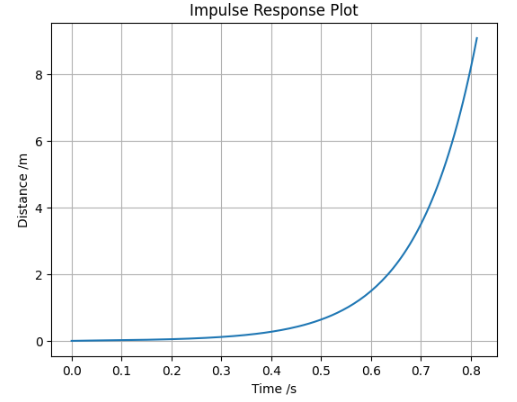
\includegraphics[width=0.65\linewidth]{Simulation/Impulse Plot no pid.png}
        \caption{Impulse response of the transfer function.}
\end{figure}

\begin{figure}[ht]
    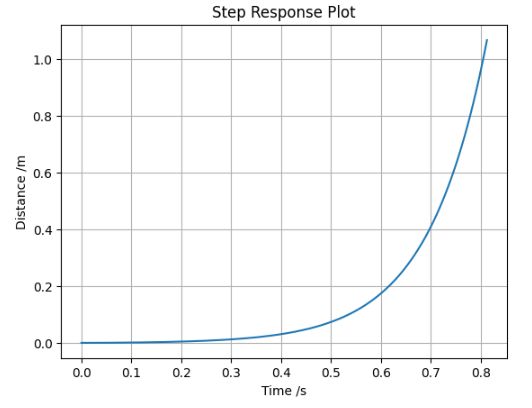
\includegraphics[width=0.65\linewidth]{Simulation/Step Plot no pid.png}
    \caption{Step response of the transfer function.}
\end{figure}

\noindent According to the Figure of the impulse response of the transfer function, When an instantaneous impact is applied to the system, the ball starts to move down the inclined plane  with increasing speed and acceleration. From the Figure of Step response of the transfer function, its situation is similar to the previous one, but with slower speed and acceleration. This illustrates the instability of a system without a controller.
\subsection*{PID plots}\hfill \\
\noindent The PID values chosen for this controller are Kp = 1135, Kd = 22.5, and Ki = 0. From the Figure of the impulse and step responses of the system, the line of impulse responses shows that the ball will move down the inclined plane between 0 and 0.1s and then upwards to a position 0.05mm from the equilibrium position. The step of impulse responses shows that when a constant force is applied to the system, the ball will move down the inclined plane and stabilise at a distance of 2.1mm from the equilibrium position. Therefore, the system is BIBO
stable, and it can be seen that the controller has a good control effect.
\begin{figure}[ht]
    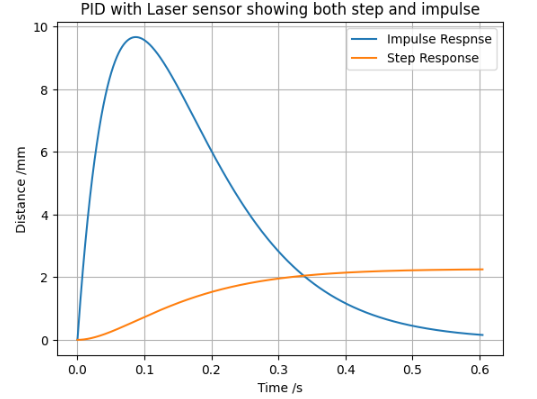
\includegraphics[width=0.65\linewidth]{Simulation/PID + Laser Both Step and Impulse plot.png}
    \caption{The impulse and step responses of the system.}
\end{figure}







